\documentclass[a4paper]{article}

\usepackage{graphicx}
\usepackage{amsmath,amssymb}
\usepackage{minted}
\usepackage{multirow}
\usepackage{float}
\usepackage{todonotes}
\usepackage{forest}
\usepackage{xstring}
\usepackage{xcolor}
\usepackage[most]{tcolorbox}
\usepackage{xparse}
\usepackage{natbib}
\usetikzlibrary{graphs,graphdrawing}
\usegdlibrary{layered}

% for external graphviz
\input{/home/donkarlo/Dropbox/repo/nd_language_ai_project/src/nd_language_ai/formal/computer/programming/tex/latex/code_clips/external_graphviz.tex}

% for tags
\input{/home/donkarlo/Dropbox/repo/nd_language_ai_project/src/nd_language_ai/formal/computer/programming/tex/latex/part/control_sequence/kind/semtag/semtag.tex}

% for links
\input{/home/donkarlo/Dropbox/repo/nd_language_ai_project/src/nd_language_ai/formal/computer/programming/tex/latex/code_clips/seehere.tex}

\title{Anomally and novelty detection}
\date{}
\author{Mohammad Rahmani}

\begin{document}

   \maketitle
   Novelty is the continous presitance of neural responses of populations of neurons

   The main question that the agent tries to answer here is can I rebuild what has happened to me with the language components that I have or is the time to introduce a new component(Phonem, word, ...)

   The goal of this section is to detect novelty from noisy data and build new language parts from it. the inputs to the language model built in online learning are

   \section{Calculation of graded potentials(EPSPs and IPSPs) in sensory neurnos}
      Upon presence of a  sensory observation the following process will be used to assign value and sign to grade dpotentials according to their Wassertein distance between the observation and the clsuters learned in training phase
      \begin{figure}[H]
         \centering
         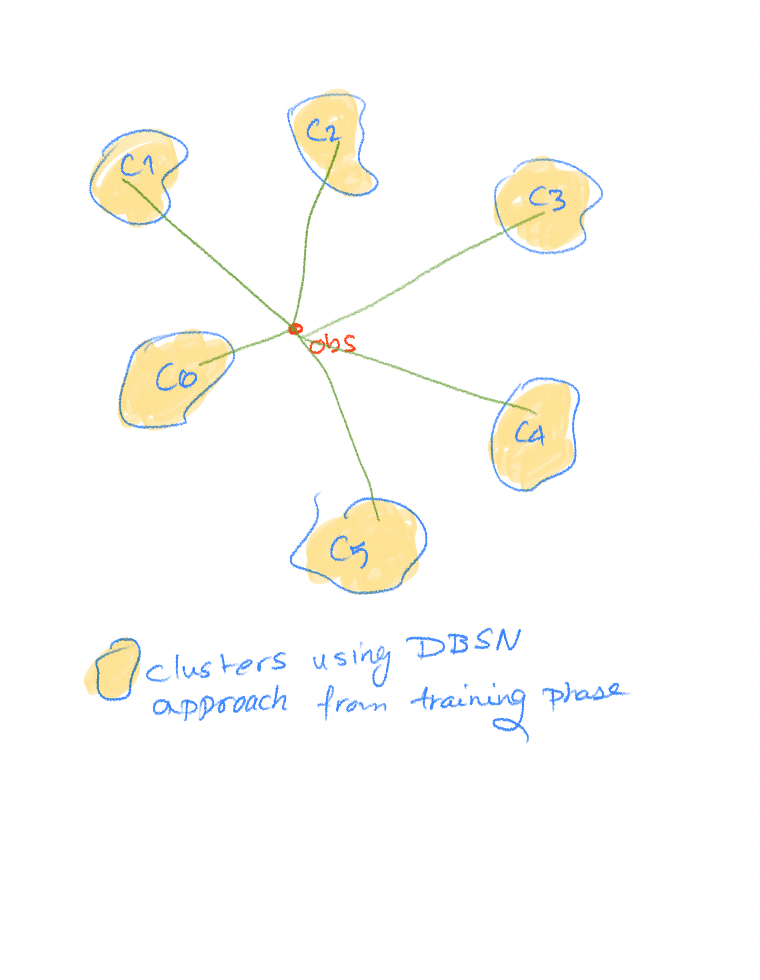
\includegraphics[width=0.9\textwidth]{ipsp_epsp_determination.png}
      \end{figure}
      Let $\mathbf{x}$ denote the current point observation, and let the $k$th learned class $C_k$ contain $N_k$ observations,

      \[
      C_k
      =
      \left\{
      \mathbf{z}_{k,1},
      \mathbf{z}_{k,2},
      \ldots,
      \mathbf{z}_{k,N_k}
      \right\},
      \]

      where $\mathbf{z}_{k,j}$ denotes the $j$th observation belonging to class $C_k$.

      The empirical probability distribution representing class $C_k$ is

      \[
      \mu_k
      =
      \frac{1}{N_k}
      \sum_{j=1}^{N_k}
      \delta_{\mathbf{z}_{k,j}},
      \]

      where $\delta_{\mathbf{z}_{k,j}}$ denotes the Dirac measure concentrated at
      $\mathbf{z}_{k,j}$. Similarly, the point observation $\mathbf{x}$ is represented by the Dirac measure $\delta_{\mathbf{x}}$.

      The point-to-class $p$-Wasserstein distance is denoted by
      $d_k(\mathbf{x})$ and is defined as

      \[
      d_k(\mathbf{x})
      =
      W_p\!\left(
      \delta_{\mathbf{x}},
      \mu_k
      \right)
      =
      \left(
      \frac{1}{N_k}
      \sum_{j=1}^{N_k}
      \left\|
      \mathbf{x}
      -
      \mathbf{z}_{k,j}
      \right\|_2^p
      \right)^{1/p}.
      \]

      For the second-order Wasserstein distance used in this research,

      \[
      \boxed{
      d_k(\mathbf{x})
      =
      W_2\!\left(
      \delta_{\mathbf{x}},
      \mu_k
      \right)
      =
      \sqrt{
      \frac{1}{N_k}
      \sum_{j=1}^{N_k}
      \left\|
      \mathbf{x}
      -
      \mathbf{z}_{k,j}
      \right\|_2^2
      }
      }.
      \]

      Therefore, $d_k(\mathbf{x})$ represents the Wasserstein distance between the current point observation $\mathbf{x}$ and the empirical distribution of class $C_k$. In this particular point-to-empirical-distribution case, it is equal to the root mean squared Euclidean distance from $\mathbf{x}$ to all observations belonging to $C_k$.

   \section{Neurons which are specifically activated}
      \begin{itemize}
         \item State neurons (results of clustering in training)
         \item Transformer (Grandmother neuron for timewise prediction). There is a trained transformer for each state level
         \item Kalmman filter (Grandmother neuron, diverging neural circuit to propgate among the time axis in all abstraction levels. Kalman filter works with intensity change neuron)
         \item Particle filter (Grandmother neuron, converging neural circuit upward in the abstraction hierarchy axis, particle filter works with change internsity sensory neuron)
         \item Language
      \end{itemize}

   \section {Observation and evidence flow}
      \begin{itemize}
         \item Sensor modality intensity values
         \item Sensor modality intensity change value
         \item Kalman filter at lowest level
         \item Particle filter at each level
      \end{itemize}

   \section{Evidence data flow}
      \subsection{At time axis:}

         \begin{figure}[H]
            \centering
            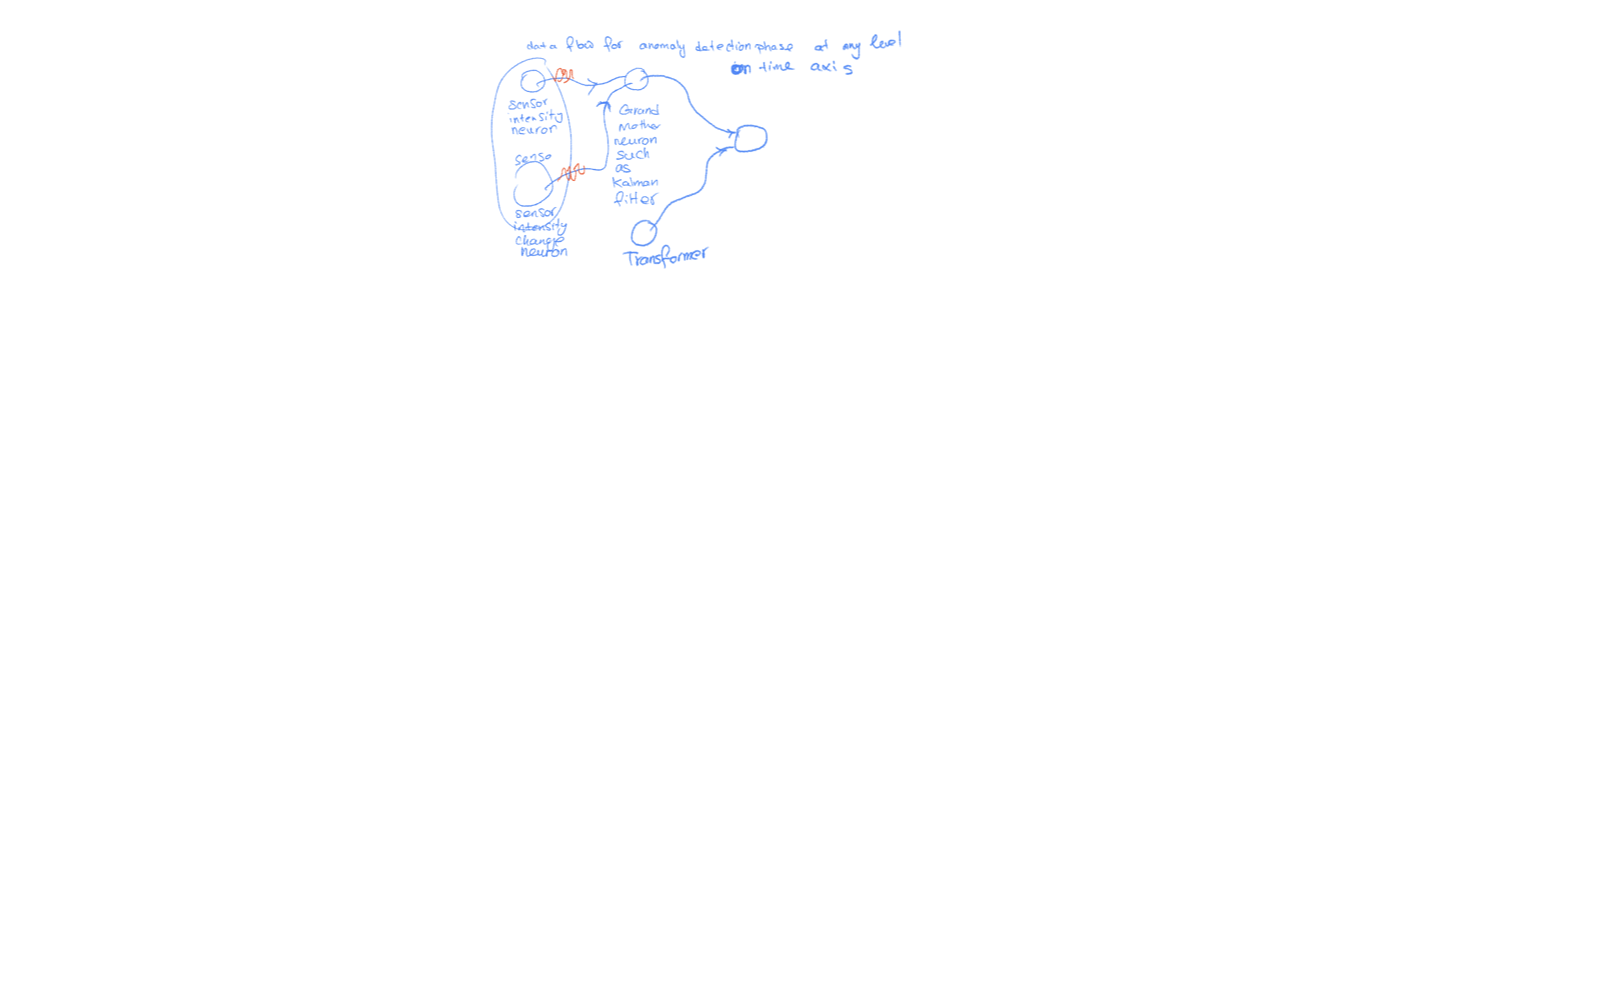
\includegraphics[width=0.9\textwidth]{data_flow_time_axis.png}
         \end{figure}

      \subsection{At concept level}
         \begin{figure}[H]
            \centering
            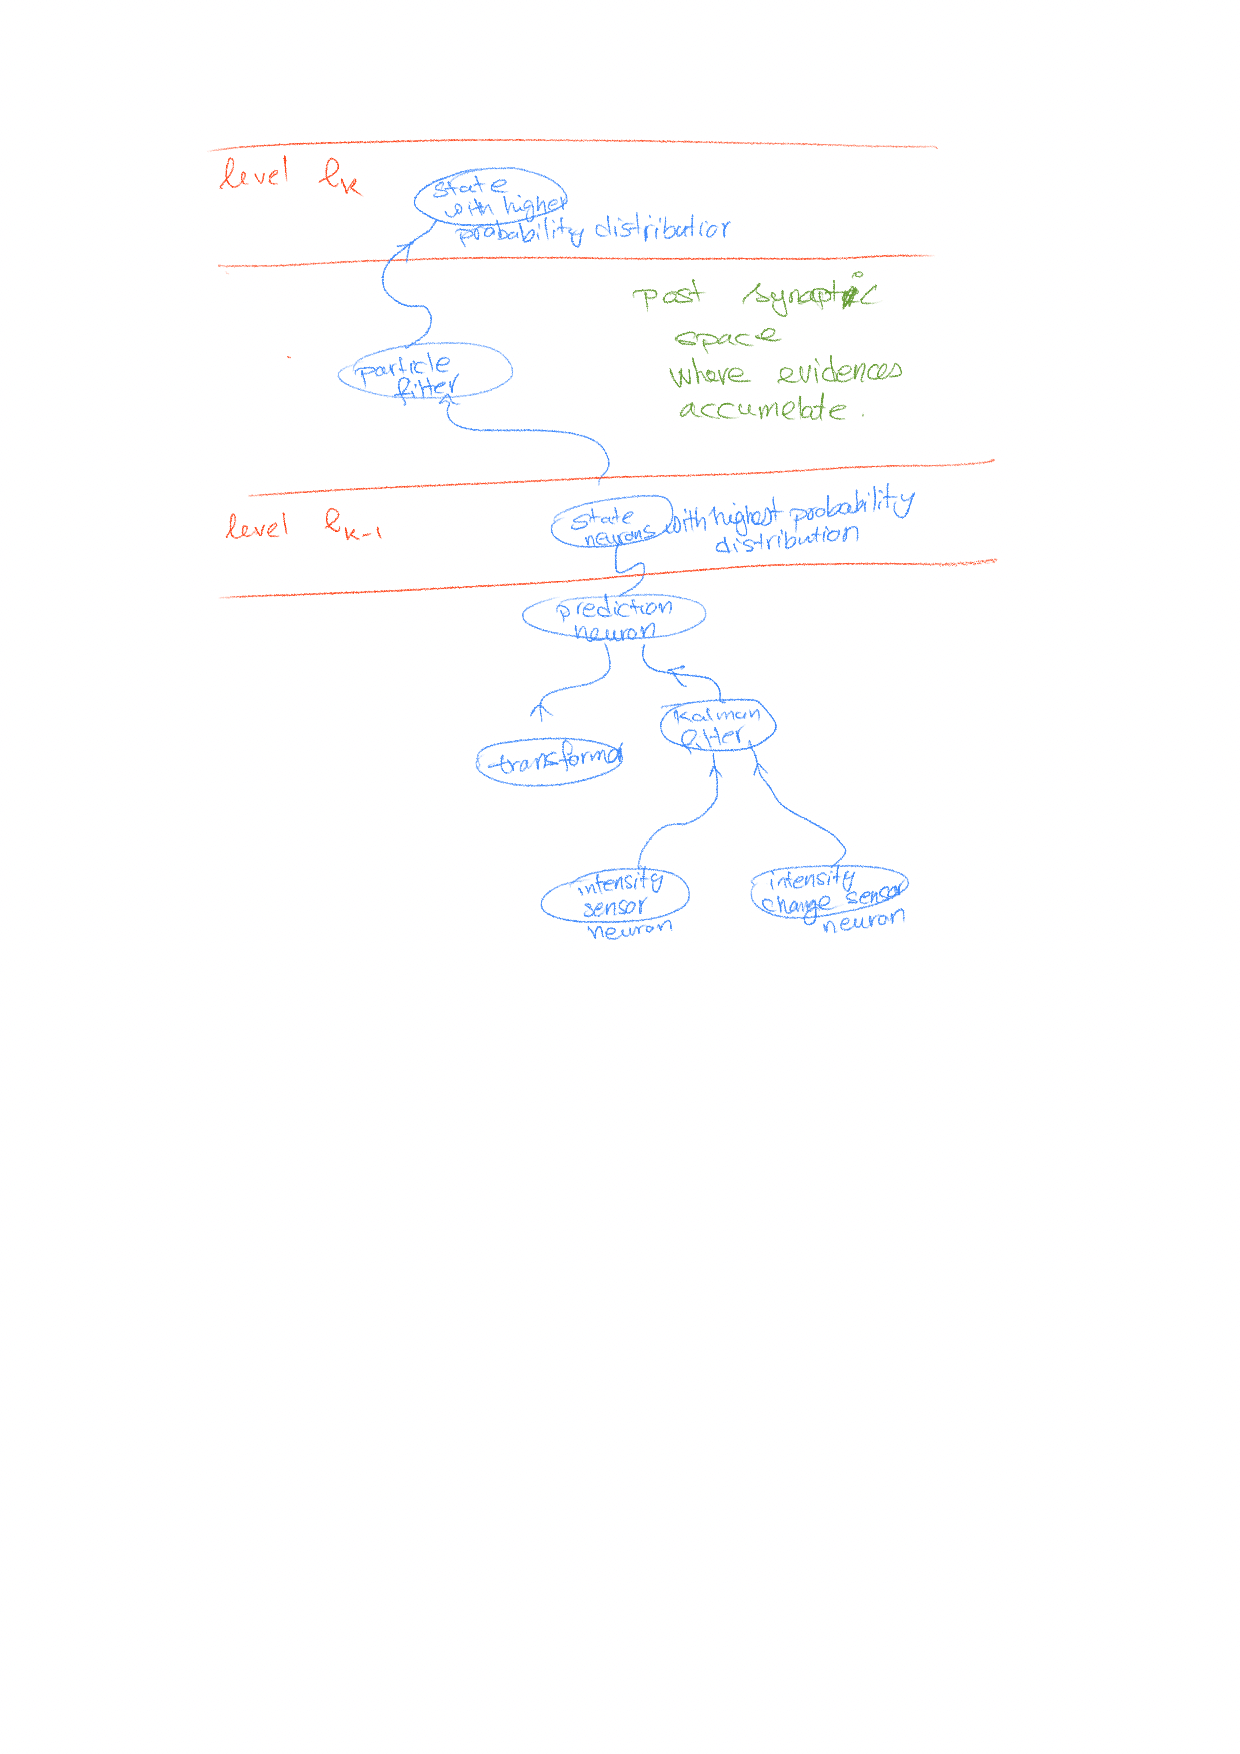
\includegraphics[width=0.9\textwidth]{data_flow_semantic_axis.png}
         \end{figure}
   \section{Discrepency detection}
      In all phases a statistical distrinbution is being assigned to the state space. In this research directed gaussian Wassersetin distance \cite{dowson-1982-the-frechet-distance-between-multivariate-normal-distributions} or \seeherefooter{/nd_math_learning_project/src/probability/distribution/discrepency/kind/distance/kind/wasserstein/gaussian/gaussian.tex} to measure the sttaistical distance between estimated current state and predicted state.



      The term \emph{directed} refers to assigning a direction to the scalar Wasserstein distance using the displacement between the two distribution means.
      Given the mean difference $\mathbf{d}=\boldsymbol{\mu}_1-\boldsymbol{\mu}_2$, its normalized direction is $\hat{\mathbf{d}}=\mathbf{d}/|\mathbf{d}|_2$.
      The directed Wasserstein vector is therefore defined as $\mathbf{v}_W=W_2(P,Q)\hat{\mathbf{d}}$, whose magnitude equals the Wasserstein distance while its direction follows the mean displacement.




      \subsection{Reason to use wasserstein distance}
         \begin{itemize}
            \item When the two distributions are points (their covariance matrix is very close to 0), then Wasserstein gives a value very close to Euclidean distance
            \item when one is a distribution and the other is a point, it still produces a value
            \item It is a metric, so unlike Kullbackleibler, distance(A,B) = distance(B,A)
         \end{itemize}
         \[
         P_1
         =
         \mathcal{N}
         \left(
         \mu_1,
         \Sigma_1
         \right)
         \qquad
         P_2
         =
         \mathcal{N}
         \left(
         \mu_2,
         \Sigma_2
         \right)
         \]

         \[
         W_2^2
         \left(
         P_1,
         P_2
         \right)
         =
         \sqrt{
         \left\lVert
         \mu_1 - \mu_2
         \right\rVert_2^2
         +
         \operatorname{Tr}
         \left(
         \Sigma_1
         +
         \Sigma_2
         -
         2
         \left(
         \Sigma_2^{1/2}
         \Sigma_1
         \Sigma_2^{1/2}
         \right)^{1/2}
         \right)}
         \]


      \subsection{Interpretation}
         If we consider the two gaussian ditributions as two mass piles, how much effort does it take to move one pile to the other.


   \section{Threshold calculation} \label{anomaly_calculation}
      \begin{enumerate}
         \item Breaking an event-specific-knowledge sensory data into periods
         \item Split the periods into train-test
         \item take $\mu + n \times \sigma$ anomaly values as the threshold
      \end{enumerate}

   \section{Anomaly detection}
      Whatever rises more than the computed threshold in section \ref{anomaly_calculation}

   \section{Novelty detection}
      \begin{algorithm}[H]
         \caption{Novelty Detection from Sensor Sequences}
         \begin{algorithmic}[1]
            \Require Preprocessed sensor sequence $X = \{x_1, x_2, \dots, x_T\}$
            \Require Trained predictive model $f_{\theta}$
            \Ensure Novelty threshold $\tau = \{y_1, y_2, \dots, y_T\}$
            \Ensure Novelty scalar value


            $Y = \{y_1, y_2, \dots, y_T\}$
            \State \Return $Y$
         \end{algorithmic}
      \end{algorithm}



      \bibliographystyle{plainnat}
      \bibliography{/home/donkarlo/Dropbox/repo/nd_shared_research/bibliography/bibliography.bib}

\end{document}